\documentclass[11pt]{beamer}

\usetheme{metropolis}

\usepackage{graphicx}
\usepackage{physics}
\usepackage{adjustbox}
\usepackage{caption}
\usepackage{chemformula}
\usepackage{quoting}
\usepackage[style=chem-angew,backend=bibtex]{biblatex}
\bibliography{references}
%
% Choose how your presentation looks.
%
% For more themes, color themes and font themes, see:
% http://deic.uab.es/~iblanes/beamer_gallery/index_by_theme.html
%
\mode<presentation>
{
  \usetheme{default}      % or try Darmstadt, Madrid, Warsaw, ...
  \usecolortheme{default} % or try albatross, beaver, crane, ...
  \usefonttheme{default}  % or try serif, structurebold, ...
  \setbeamertemplate{navigation symbols}{}
  \setbeamertemplate{caption}[numbered]
  \setbeamerfont{footnote}{size=\tiny}
} 

\usepackage[english]{babel}
\usepackage[utf8]{inputenc}
\graphicspath{{image/}}

\AtBeginSection[]{
\begin{frame}{Outline}
  \tableofcontents[currentsection]
\end{frame}
}

\title{Chapter 7: Electron Structure of the Atom}
\institute{Chemistry Department, Cypress College}
\date{October 24, 2022}

\begin{document}

\begin{frame}
  \titlepage
\end{frame}

\begin{frame}{Class Announcements}
  \textbf{Lab}
  \begin{itemize}
  \item Experiment 16 - Electromagnetic Energy and Spectroscopy
  \item Review - Wavelength and Excitation of Electron
  \item Reminder - Need $70\%$ of laborator points to pass
    the course
  \end{itemize}

  \textbf{Lecture}
  \begin{itemize}
  \item Review the Exam and proposal
  \item Ch 7+8 - Electronic Structure of Atom and Chemical Bonding
  \item Go over homework 8 (EC for students who present)
  \item Quiz and Homework assignment released Fri, Nov 4th at 3pm
  \end{itemize}
\end{frame}

\begin{frame}{Making the Most of It}

  Questions to consider:
  \begin{itemize}
  \item Why am I taking this course?
  \item What would I like to achieve?
  \item What methods/tools/resources work for me?
  \end{itemize}

  Your feedback, questions, participation are vital:
  \begin{itemize}
  \item Attend lectures and discussions, if possible
  \item Give on-going feedback to instructors through facial expression,
    emojis, chat, email, during office hours etc.
  \item Fill out evaluations
  \item Own your education
  \item Be proactive, do not hesitate to speak up or get help
  \end{itemize}

\end{frame}

\section{Review: Atomic Spectra and Quantum Chemistry}

\begin{frame}{Atomic Spectra}
  \centering
  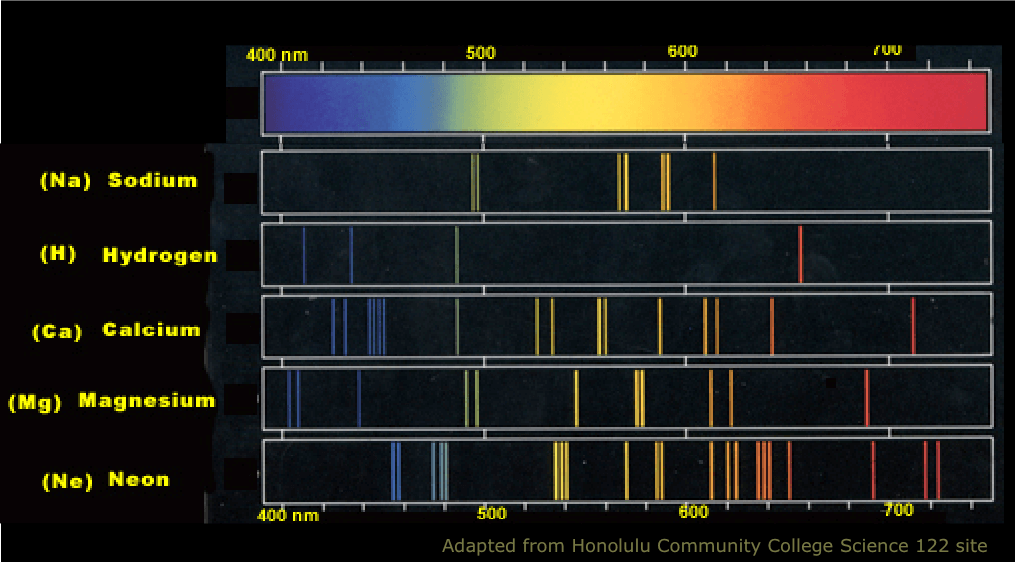
\includegraphics[width=0.85\linewidth]{cont_line}
  \begin{itemize}
  \item Continuous spectra is given at the top and
    discrete lines are emitted by atoms
  \item \textbf{Q:} Why are there discrete lines for
    the atomic spectra?
  \end{itemize}
\end{frame}

\begin{frame}{Introduction to Quantum Chemistry}
  \textbf{Schr\"{o}dinger's Cat} - Thought Experiment
  \begin{center}
    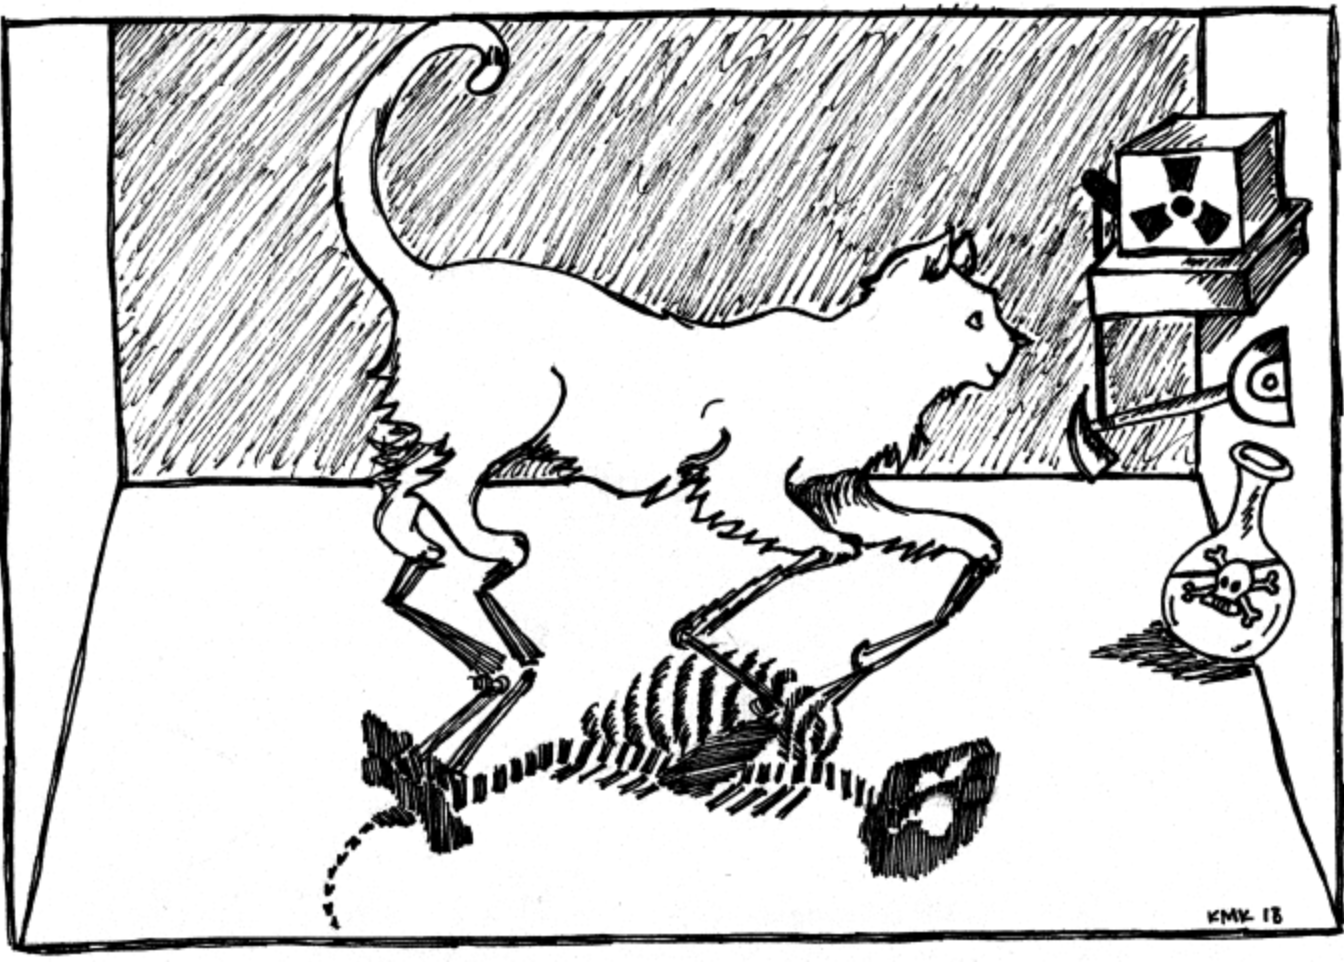
\includegraphics[width=0.65\linewidth]{schor_cat}
  \end{center}

  The world that we know is deterministic, however, dealing
  with electrons or small subatomic particles, we have to think
  of it in terms of probabilities
\end{frame}

\begin{frame}{The Wavefunction $\Psi$}
  \textbf{Schr\"{o}dinger's Equation}
  \begin{equation}
    \hat{H}\Psi = E\Psi
  \end{equation}
  where $\hat{H}$ is the Hamiltonian, $E$ is the energy,
  and $\Psi$ is the wavefunction
  \begin{itemize}
  \item Equation that explain everything about your system
  \item Chemical and physical properties can be determined
    from the $\Psi$
  \end{itemize}
\end{frame}

\begin{frame}{Atomic Orbitals}
  \centering
  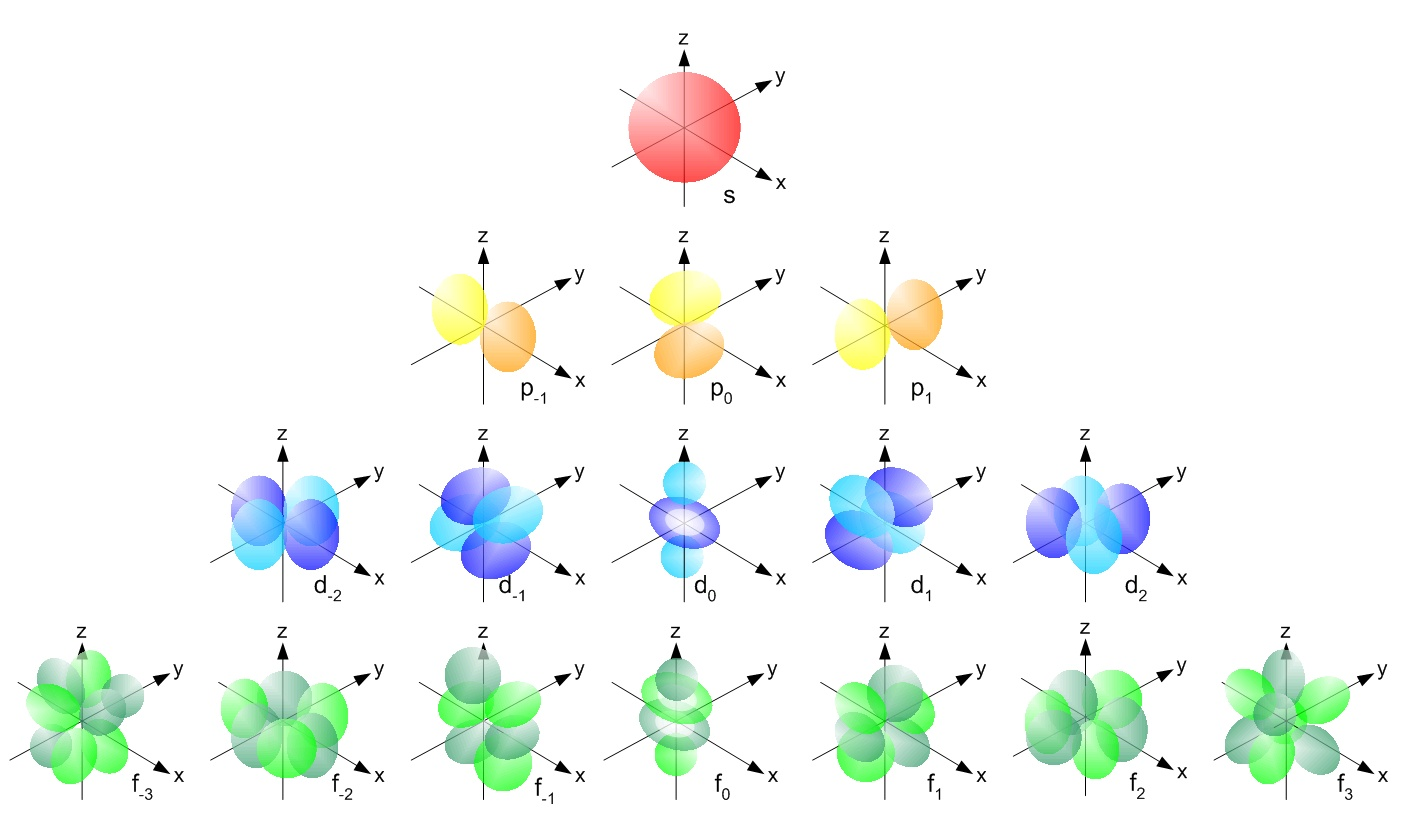
\includegraphics[width=\linewidth]{single_elect_orb}
\end{frame}

\section{Rydberg Formula}

\begin{frame}{Rydberg Formula}
  Mathematical formula to compute the wavelength between energy
  levels $n$ of a hydrogen atom

  \centering
  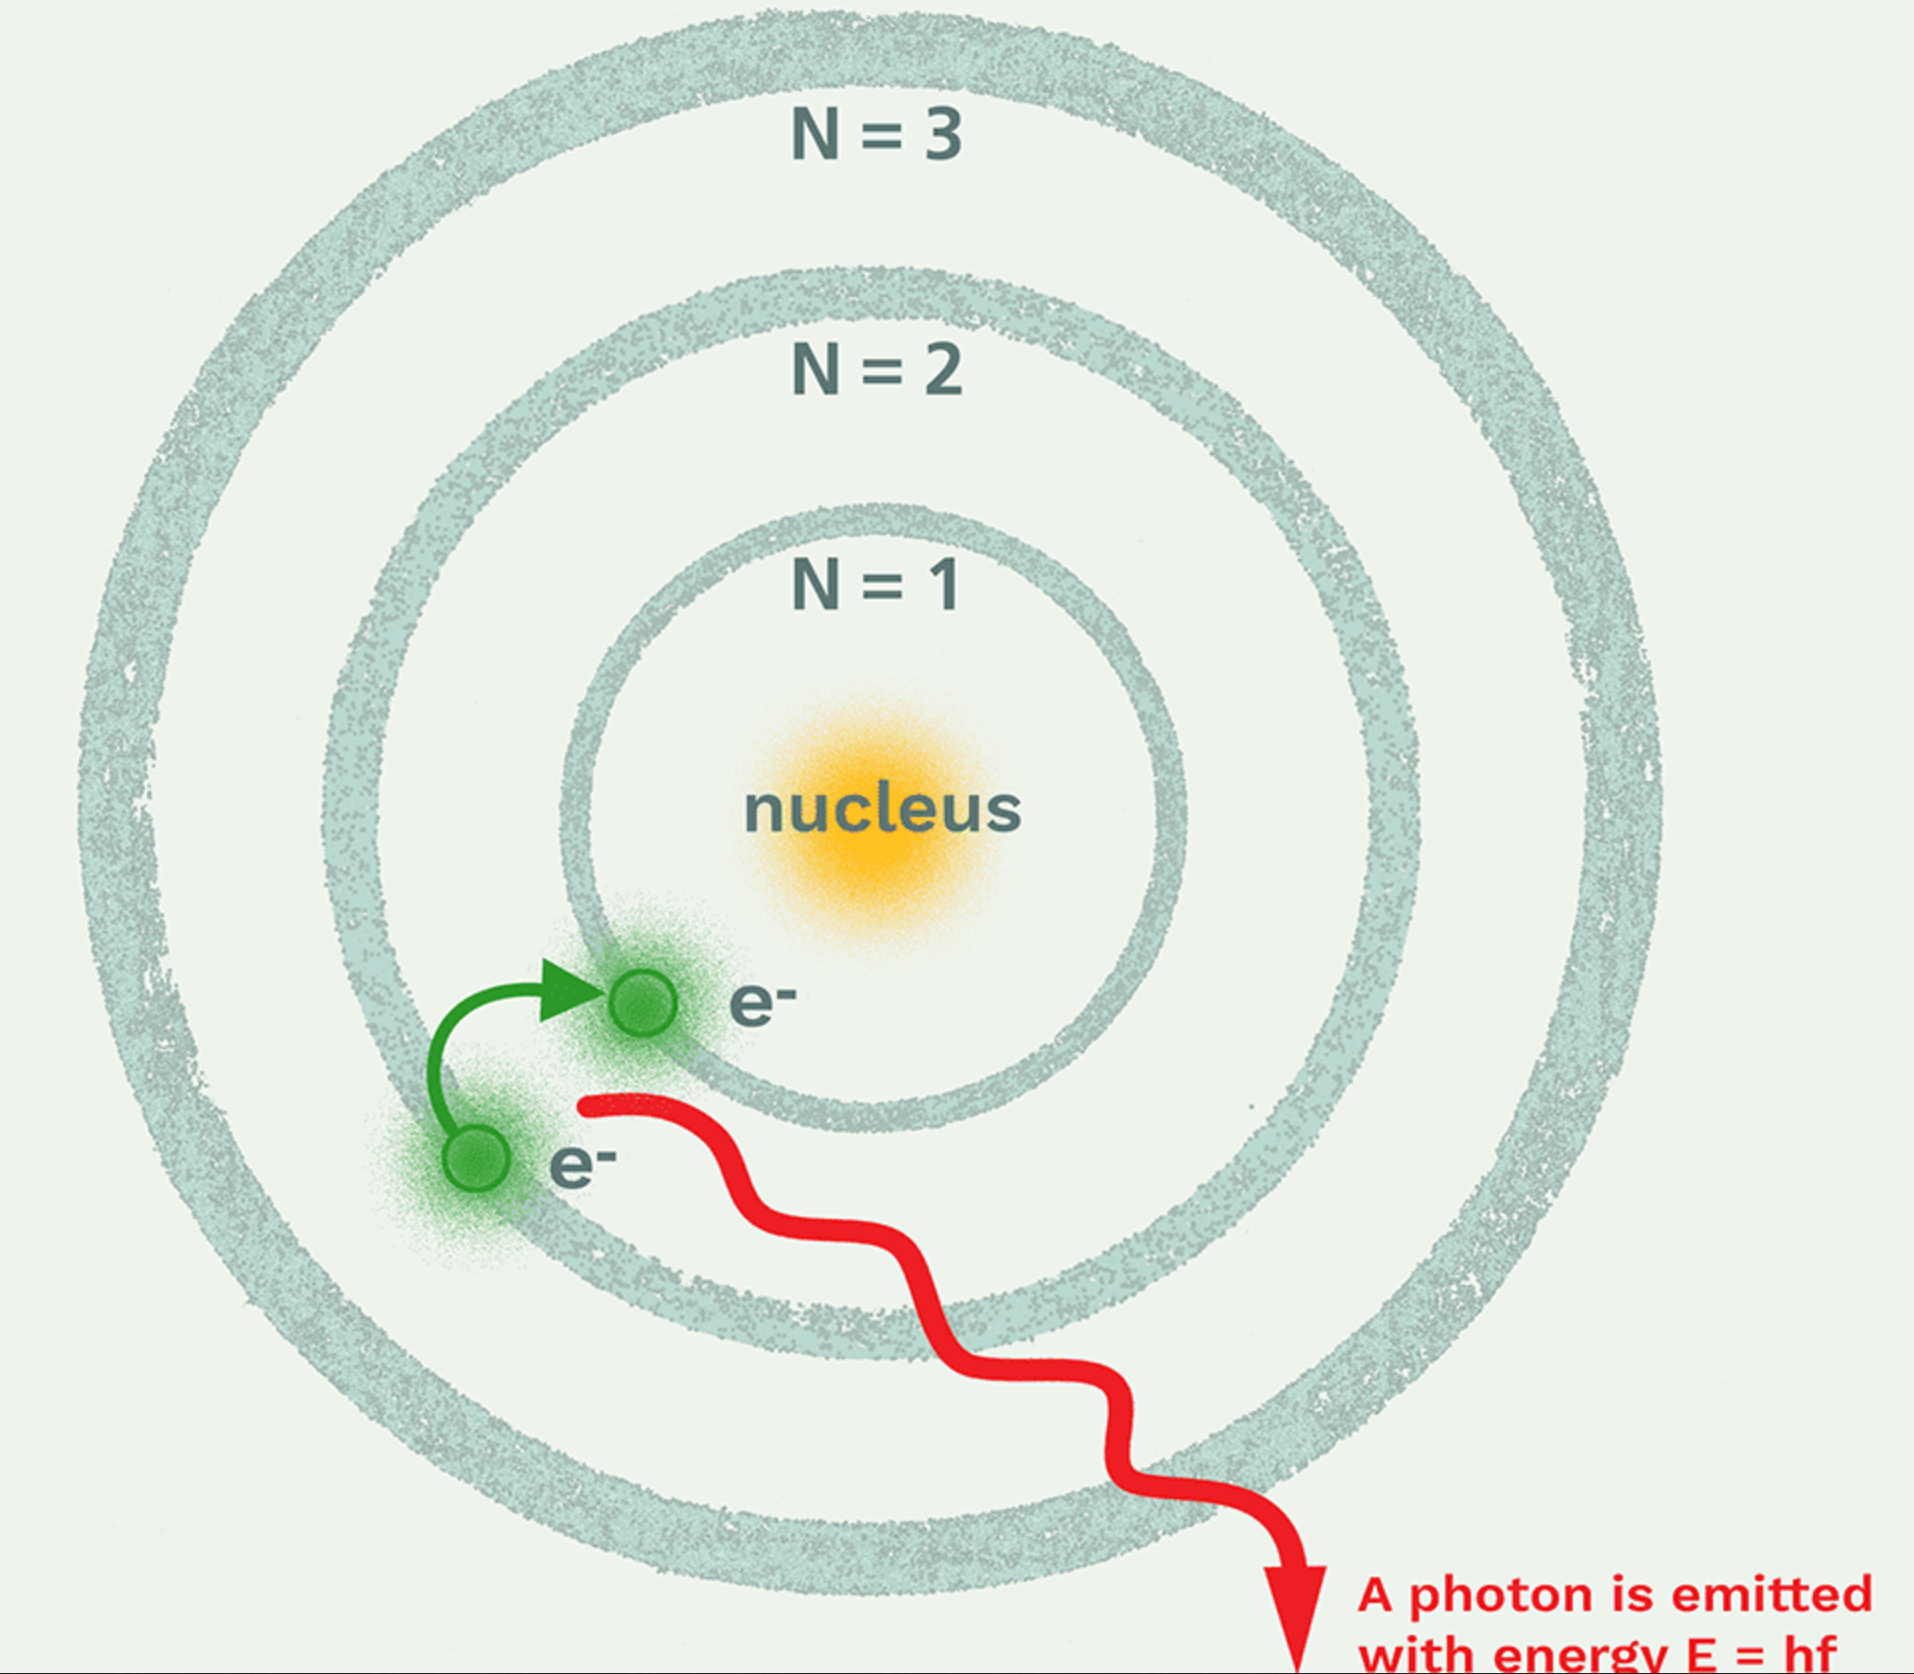
\includegraphics[width=0.55\linewidth]{bohr_model}
\end{frame}

\begin{frame}{Rydberg Formula}
  \begin{equation}
    \frac{1}{\lambda} = R\Bigg(\frac{1}{n_f^2} - \frac{1}{n_i^2}\Bigg)
  \end{equation}
  where $n_f$ and $n_i$ are the final and initial energy state,
  $\lambda$ is the wavelength, and $R$ is the Rydberg constant
  ($1.097\times 10^7$ m$^{-1}$)
\end{frame}

\begin{frame}{Practice: Using Rydberg Formula}
  Calculate the wavelength of light emitted when a hydrogen atom relaxes
  from $n = 6$ to $n = 2$. Is this light in the visible region of
  electromagnetic spectrum? If so, what color is it?
  \onslide<2->{
  \begin{center}
    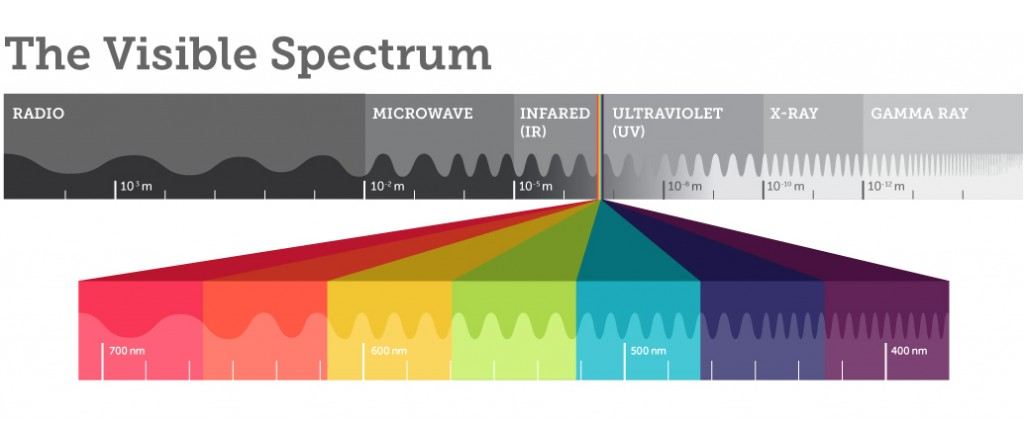
\includegraphics[width=1\linewidth]{visible_light}
  \end{center}
  }
  \vfill
\end{frame}

\begin{frame}{Practice: Using Rydberg Formula}
  What is the energy of the wavelength when a hydrogen atom relaxes
  from $n = 6$ to $n = 2$?
  \vfill
\end{frame}

\section{Periodicity of Electron Configurations}

\begin{frame}{Atomic Orbitals}
  \centering
  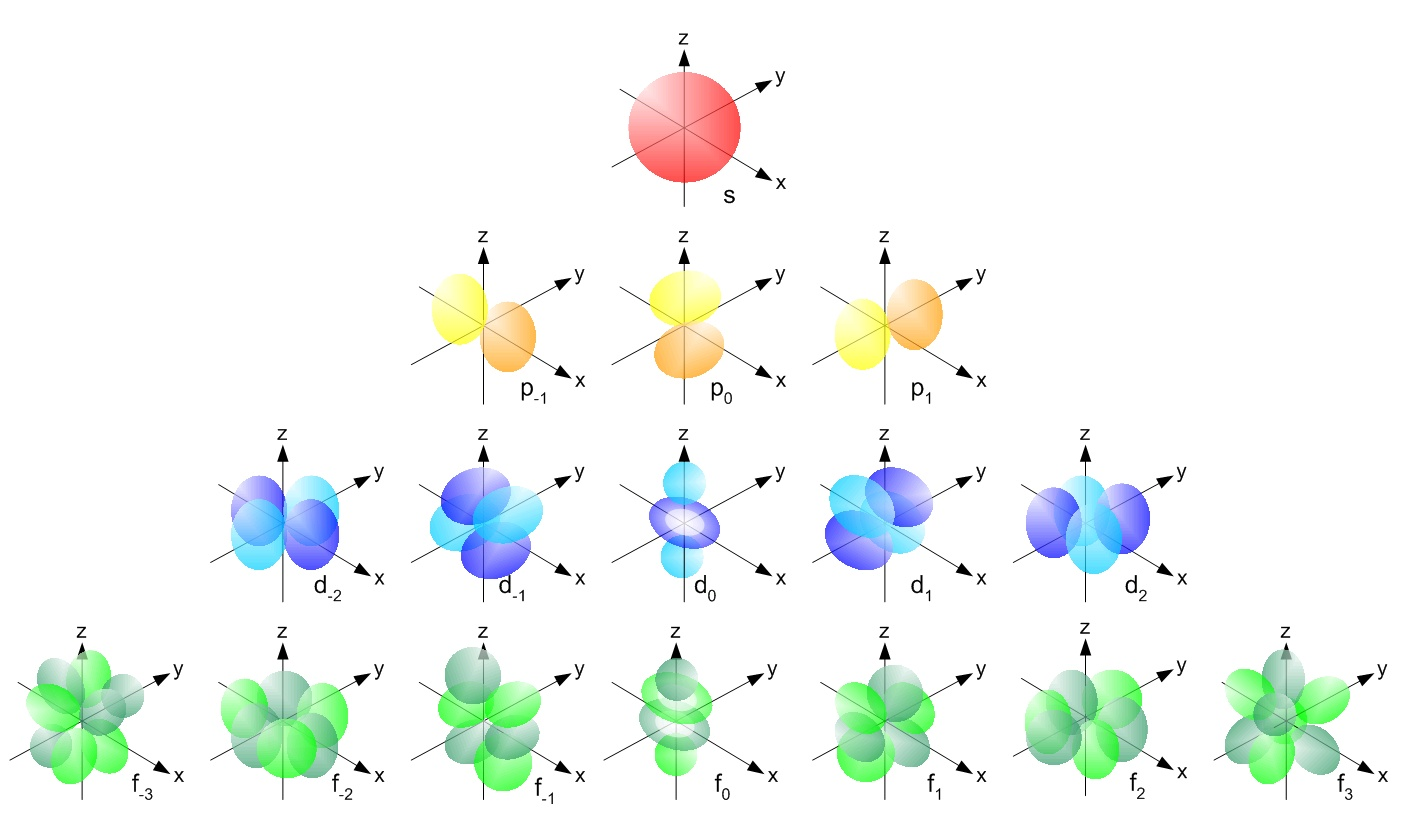
\includegraphics[width=0.8\linewidth]{single_elect_orb}
  \begin{itemize}
  \item Specific orbitals occupy certain \textbf{principal energy level} e.g.
    $n = 1, 2, 3, \cdots$
  \item Basis in which atoms form bond; atomic orbitals combine to make
    molecular orbitals
  \end{itemize}
\end{frame}

\begin{frame}{Orbital Diagram - Hydrogen}
  \centering
  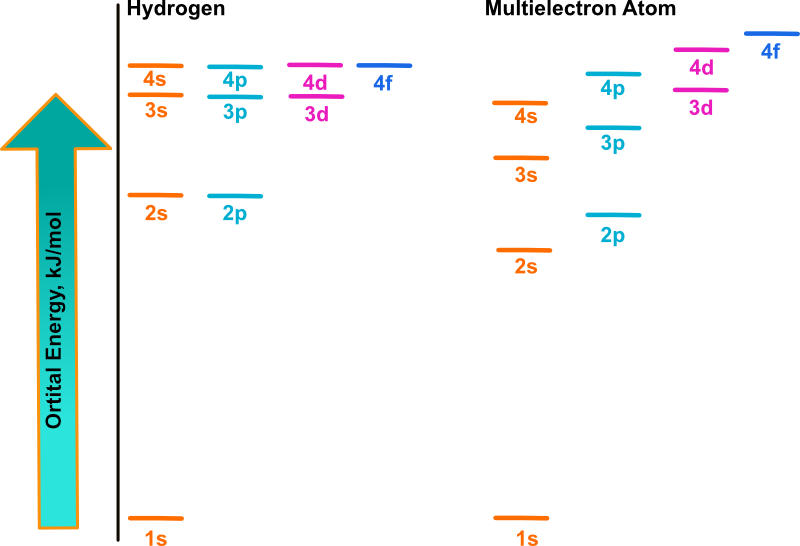
\includegraphics[scale=1.5,trim={0 0 1.2in 0},clip]{orbital_energy}
\end{frame}

\begin{frame}{Orbital Diagram - Multielectron Element}
  \textbf{Q:} What do notice about the relative atomic orbital energies?
  
  \centering
  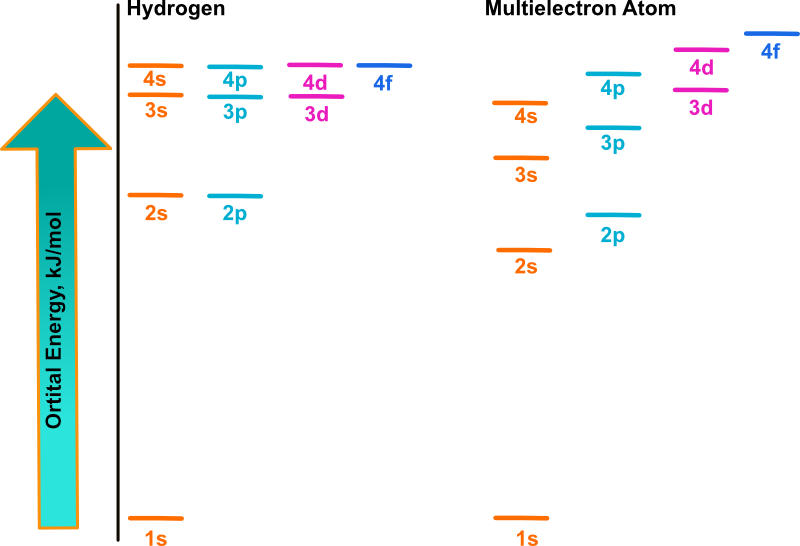
\includegraphics[scale=1.3]{orbital_energy}
\end{frame}

\begin{frame}{Principles for Filling Atomic Orbitals}
  \textbf{Aufbau principle} - electrons fill an orbital starting with
  the lowest energy level

  \textbf{Pauli exclusion princple} - No two electrons with the same
  spin can occupy the same orbital

  \textbf{Hund's Rule} - Maximize the number of unpaired electrons
\end{frame}

\begin{frame}{Examples: Write Electron Configurations}
  \textbf{H}
  \vspace{0.25in}
  
  \textbf{He}
  \vspace{0.25in}
  
  \textbf{Li}
  \vspace{0.25in}

  \textbf{Na}
\end{frame}

\begin{frame}{Purpose of Electron Configurations}
  \begin{itemize}
  \item Outermost shell is referred to as the valence
    electrons (\textbf{Q:} What is special about valence electrons?)
  \item Innermost shell is the core electrons
  \item Predicts stability of the atom e.g. unfilled orbitals
    indicate instability
  \item Make predictions how elements react forming new chemical
    compounds
  \end{itemize}
\end{frame}

\begin{frame}{Practice: Writing Electron Configurations}
  \textbf{F}
  \vspace{0.25in}
  
  \textbf{F$^-$}
  \vspace{0.25in}
  
  \textbf{Na$^+$}
  \vspace{0.25in}

  \textbf{Fe}  
\end{frame}

\end{document}
